\chapter{Basic Data Representation}
\label{chap:basic_data_representation}

\begin{figure}[ht]
	\hfill
	\begin{minipage}{0.5\textwidth}
		\centering
		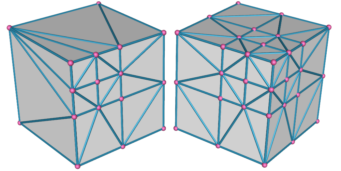
\includegraphics{VTKTextbook-48}\\
		\caption*{\texttt{Compatible tessellations.}}
	\end{minipage}
\end{figure}

\firstletter{I}n Chapter 4 we developed a pragmatic definition of the visualization process: mapping information into graphics primitives.
We saw how this mapping proceeds through one or more steps, each step transforming data from one form, or data representation, into another.
In this chapter we examine common data forms for visualization.
The goal is to familiarize you with these forms, so that you can visualize your own data using the tools and techniques provided in this text.

\section{Introduction}
To design representational schemes for data we need to know something about the data we might
encounter. We also need to keep in mind design goals, so that we can design efficient data structures
and access methods. The next two sections address these issues.

\subsection{Characterizing Visualization Data}

Since our aim is to visualize data, clearly we need to know something about the character of the data. This knowledge will help us create useful data models and powerful visualization systems. Without a clear understanding of the data, we risk designing inflexible and limited visualization systems. In the following we describe important characteristics of data. These characteristics are the discrete nature of data, whether it is regular or irregular, and its topological dimension.

First, visualization data is discrete. This is because we use digital computers to acquire, ana lyze, and represent our data, and typically measure or sample information at a finite number of points. Hence, all information is necessarily represented in discrete form. 

Consider visualizing the simple continuous function $y = x6 2$. If we are using a conventional digital computer, we must discretize this equation to operate on the data it represents (we are ignoring symbolic/analog computers and methods). For example, to plot this equation we would sample the function in some interval, say $(-1,1)$, and then compute the value y of the function at a series of discrete points $x = x_i$ in this interval. The resulting points $((x_0,y_0), (x_1,y_1), (x_2,y_2), ... (x_n,y_n))$ connect the points with straight line segments. Thus, our (continuous) data is represented by a discrete sampling.

Because of the discrete character of the data we do not know anything about regions in between data values. In our previous example, we know that data is generated from the function $y = x^2$, but, generally speaking, when we measure and even compute data, we cannot infer data values between points. This poses a serious problem, because an important visualization activity is to determine data values at arbitrary positions. For example, we might probe our data and desire data values even though the probe position does not fall on a known point.

There is an obvious solution to this problem: interpolation. We presume a relationship between neighboring data values. Often this is a linear function, but we can use quadratic, cubic, spline, or other interpolation functions. Chapter 8: \nameref{chap:advanced_data_representation} discusses interpolation functions in greater detail, but for now suffice it to say that interpolation functions generate data values in between known points.

A second important characteristic of visualization data is that its structure may be regular or irregular (alternatively, structured or unstructured). Regular data has an inherent relationship between data points. For example, if we sample on an evenly spaced set of points, we do not need to store all the point coordinates, only the beginning position of the interval, the spacing between points, and the total number of points. The point positions are then known implicitly, which can be taken of advantage of to save computer memory.

Data that is not regular is irregular data. The advantage of irregular data is that we can represent information more densely where it changes quickly and less densely where the change is not so great. Thus, irregular data allows us to create adaptive representational forms, which can be beneficial given limited computing resources.

Characterizing data as regular or irregular allows us to make useful assumptions about the data. As we saw a moment ago, we can store regular data more compactly. Typically, we can also compute with regular data more efficiently relative to irregular data. On the other hand, irregular data gives us more freedom in representing data and can represent data that has no regular patterns.

Finally, data has a topological dimension. In our example $y = x^2$ , the dimension of the data is one, since we have the single independent variable $x$. Data is potentially of any dimension from 0D points, to 1D curves, 2D surfaces, 3D volumes, and even higher dimensional regions.

The dimension of the data is important because it implies appropriate methods for visualization and data representation. For example, in 1D we naturally use x-y plots, bar charts, or pie charts, and store the data as a 1D list of values. For 2D data we might store the data in a matrix, and visualize it with a deformed surface plot (i.e., a height field — see Exercise ***4.2***).

In this chapter and Chapter 8: \nameref{chap:advanced_data_representation}, we show how these characteristics: discrete, regular/irregular, and data dimension, shape our model of visualization data. Keep these features in mind as you read these chapters.

\begin{figure}[!htb]
	\centering
	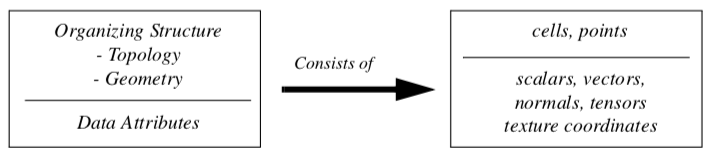
\includegraphics[width=0.8\textwidth]{Figure5-1}
	\caption{The architecture of a dataset. A dataset consists of an organizing structure, with both topological and geometric properties, and attribute data associated with the structure.}
	\label{fig:Figure5-1}
\end{figure}

\subsection{Design Criterion}

Visualizing data involves interfacing to external data, mapping into internal form, processing the data, and generating images on a computer display device. We pose the question: What form or forms should we use to represent data? Certainly many choices are available to us. The choice of representation is important because it affects the ability to interface to external data and the performance of the overall visualization system. To decide this issue we use the following design criteria:

\begin{description}

\item[Compact.] Visualization data tends to be large, so we need compact storage schemes to minimize computer memory requirements.

\item[Efficient.] Data must be computationally accessible. We want to retrieve and store data in constant time (i.e., independent of data size). This requirement offers us the opportunity to develop algorithms that are linear, or $O(n)$, in time complexity.

\item[Mappable.] There are two types of mappings. First, data representations need to efficiently map into graphics primitives. This ensures fast, interactive display of our data. Second, we must be able to easily convert external data into internal visualization data structures. Otherwise, we suffer the burden of complex conversion processes or inflexible software

\item[Minimal Coverage.] A single data representation cannot efficiently describe all possible data types. Nor do we want different data representations for every data type we encounter. Therefore, we need a minimal set of data representations that balances efficiency against the number of data types.

\item[Simple.] A major lesson of applied computation is that simple designs are preferable to complex designs. Simple designs are easier to understand, and therefore, optimize. The value of simplicity cannot be overemphasized. Many of the algorithms and data representations in this text assign high priority to this design criterion.

\end{description}

The remainder of this chapter describes common visualization data forms based on these design criteria. Our basic abstraction is the data object, a general term for the various concrete visualization data types which are the subclasses of data object. 

\section{The Data Object}

The most general form of data found in VTK is the data object. A data object can be thought of as a collection of data without any form. Data objects represent the data that is processed by the visualization pipeline (see the previous chapter and Figure ***4-2***). Taken by themselves, data objects carry little useful information. It is only when they are organized into some structure that they provide a form that we can operate on with visualization algorithms.

\section{The Dataset}

Data objects with an organizing structure and associated data attributes (Figure \ref{fig:Figure5-11}) form datasets. The dataset is an abstract form; we leave the representation and implementation of the structure to its concrete subclasses. Most algorithms (or process objects) in VTK operate on datasets.

The structure has two parts: topology and geometry. Topology is the set of properties invariant under certain geometric transformations \cite{Weiler86}. Here we consider the transformations: rotation, translation, and nonuniform scaling. Geometry is the instantiation of the topology, the specification of position in 3D space. For example, saying that a polygon is a ``triangle'', specifies topology. By providing point coordinates, we specify geometry.

Dataset attributes are supplemental information associated with geometry and/or topology. This information might be a temperature value at a point or the inertial mass of a cell.

Our model of a dataset assumes that the structure consists of cells and points. The cells specify the topology, while the points specify the geometry. Typical attributes include scalars, vectors, normals, texture coordinates, and tensors.

The definition of the structure of a dataset as a collection of cells and points is a direct consequence of the discrete nature of our data. Points are located where data is known and the cells allow us to interpolate between points. We give detailed descriptions of dataset structure and attributes in the following sections.

\section{Cell Types}

A dataset consists of one or more cells (Figure \ref{fig:Figure5-2} and Figure \ref{fig:Figure5-4}). Cells are the fundamental building blocks of visualization systems. Cells are defined by specifying a type in combination with an ordered list of points. The ordered list, often referred to as the connectivity list, combined with the type specification, implicitly defines the topology of the cell. The $x-y-z$ point coordinates define the cell geometry.

Figure \ref{fig:Figure5-3} shows one cell type, a hexahedron. The ordered list is a sequence of point ids that index into a point coordinate list. The topology of this cell is implicitly known: we know that $(8,10)$ is one of the 12 edges of the hexahedron, and that $(8,10,22,21)$ is one of its six faces.

Mathematically, we represent a cell by the symbol $C_i$. Then the cell is an ordered set of points $C_1 = {p_1, p_2,..., p_n}$ with $p_i \in P$ is a set of n-dimensional points (here $n=3$). They type of cell determines the sequence of points or cell topology. The number of points $n$ defining the cell is the \emph{size} of the cell. A cell $C_i$ ``uses'' a point $p_i$ when $p_i \in C_i$. Hence the ``use set'' $U(p_i)$ is the collection of all cells using $p_i$:

\begin{equation}\label{eq:5.1}
U(p_i) = {C_i:p_i \in C_i}
\end{equation}
\myequations{The ``use set''. }

\begin{figure}[!htb]
	\centering
	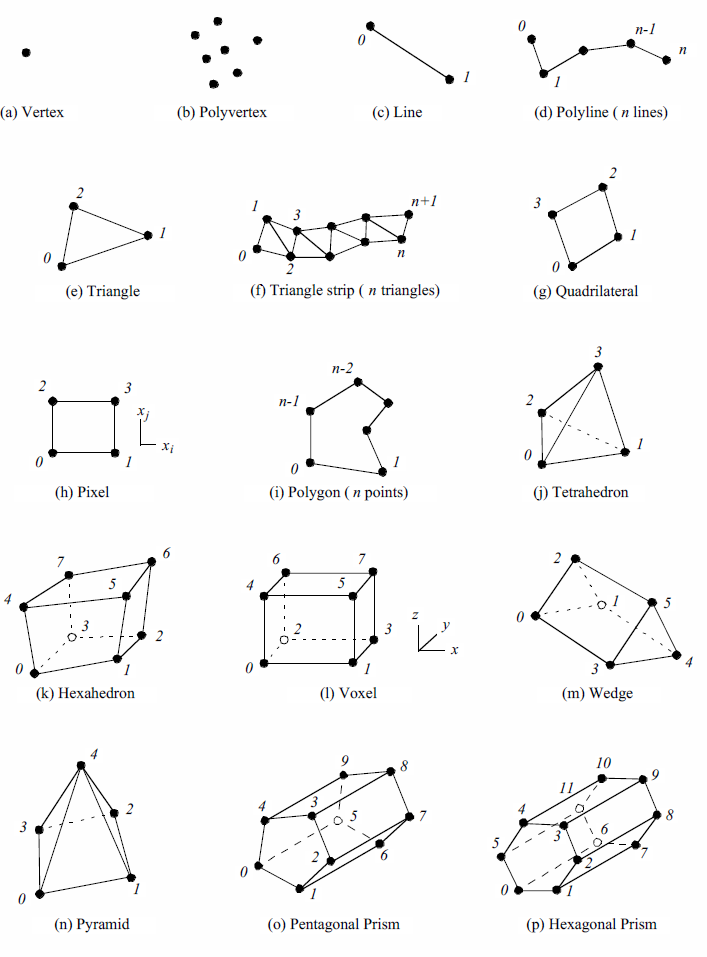
\includegraphics[width=0.8\textwidth]{Figure5-2}
	\caption{Linear cell types found in VTK. Numbers define ordering of the defining points.}
	\label{fig:Figure5-2}
\end{figure}


\begin{figure}[!htb]
	\centering
	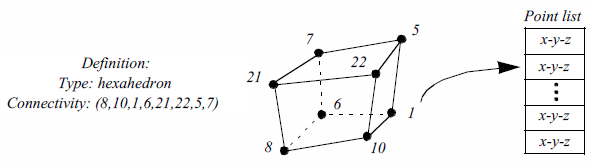
\includegraphics[width=0.8\textwidth]{Figure5-3}
	\caption{Example of a hexahedron cell. The topology is implicitly defined by the ordering of the point list. Physical generation of an image.}
	\label{fig:Figure5-3}
\end{figure}

The importance of ``uses'' and ``use sets'' will become evident in Chapter 8: \nameref{chap:advanced_data_representation} when we explore the topology of datasets.

Although we define points in three dimensions, cells may vary in topological dimension. Vertices, lines, triangles, and tetrahedron are examples of topologically 0, 1, 2, and 3-D cells, respectively, embedded in three-dimensional geometric space. Cells can also be primary or composite. Composite cells consist of one or more primary cells, while primary cells cannot be decomposed into combinations of other primary cell types. A triangle strip, for example, consists of one or more triangles arranged in compact form. The triangle strip is a composite cell because it can be broken down into triangles, which are primary cells.

Certainly there are an infinite variety of possible cell types. In the \emph{Visualization Toolkit} each cell type has been chosen based on application need. We have seen how some cell types: vertex, line, polygon, and triangle strip (\ref{fig:Figure3-19}) are used to represent geometry to the graphics subsystem or library. Other cell types such as the tetrahedron and hexahedron are common in numerical simulation. The utility of each cell type will become evident through the practice of visualization throughout this book. A description of the cell types found in the \emph{Visualization Toolkit} including their classification as linear, nonlinear, or other is given in the following sections.

\subsection{Linear Cells}

\begin{figure}[!htb]
	\centering
	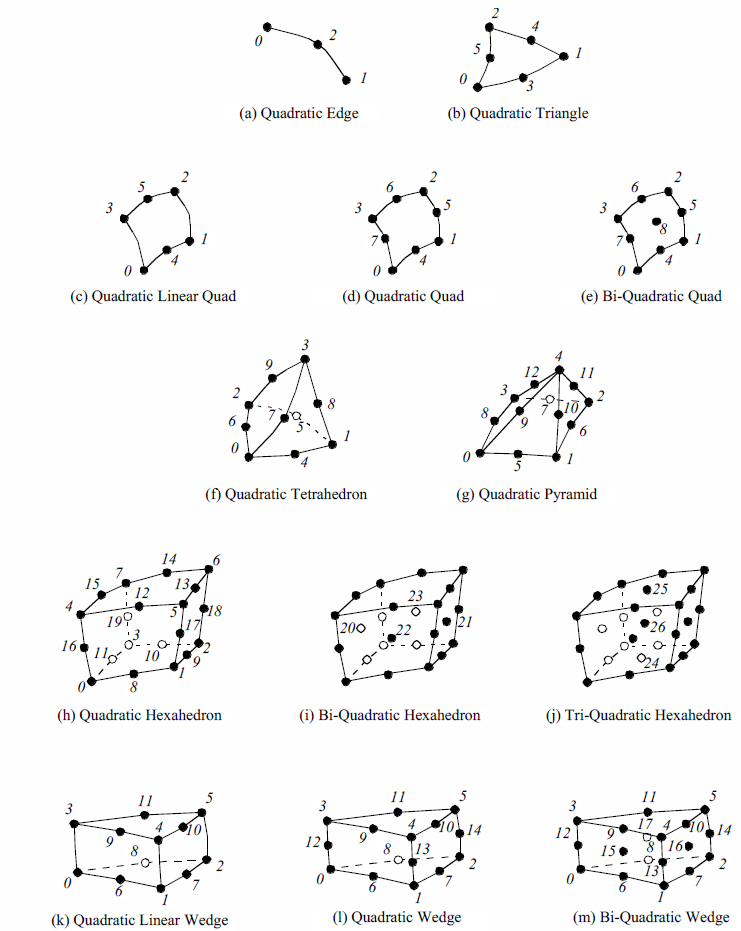
\includegraphics[width=0.8\textwidth]{Figure5-4}
	\caption{Nonlinear cell types found in VTK.}
	\label{fig:Figure5-4}
\end{figure}


\begin{figure}[!htb]
	\centering
	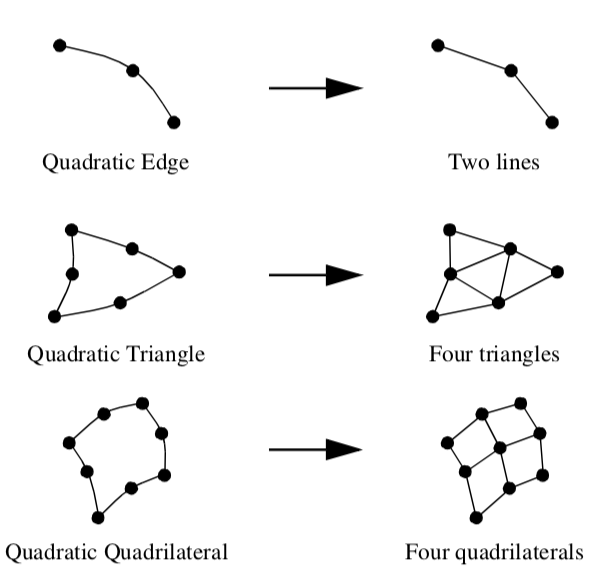
\includegraphics[width=0.8\textwidth]{Figure5-5}
	\caption{Decomposing quadratic nonlinear cells into linear cells. The quadratic tetrahedron is tessellated into six linear tetrahedron; the quadratic hexahedron is tessellated into eight linear hexahedra. Note that some tessellations require the addition of new points. In VTK, a cell adaptor framework is available for tessellating cells with basis functions of arbitrary complexity, see Chapter 8: \nameref{chap:advanced_data_representation} for more information.}
	\label{fig:Figure5-5}
\end{figure}

\begin{figure}[!htb]
	\centering
	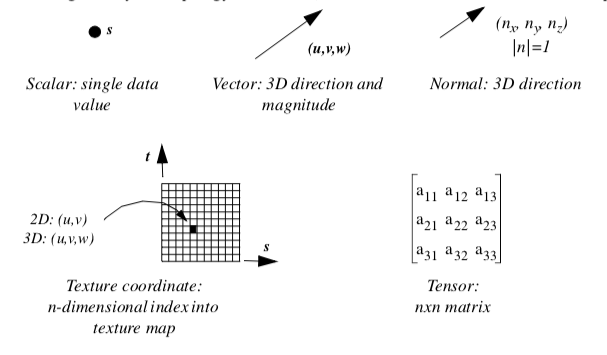
\includegraphics[width=0.8\textwidth]{Figure5-6}
	\caption{Attribute data.}
	\label{fig:Figure5-6}
\end{figure}

\begin{figure}[!htb]
	\centering
	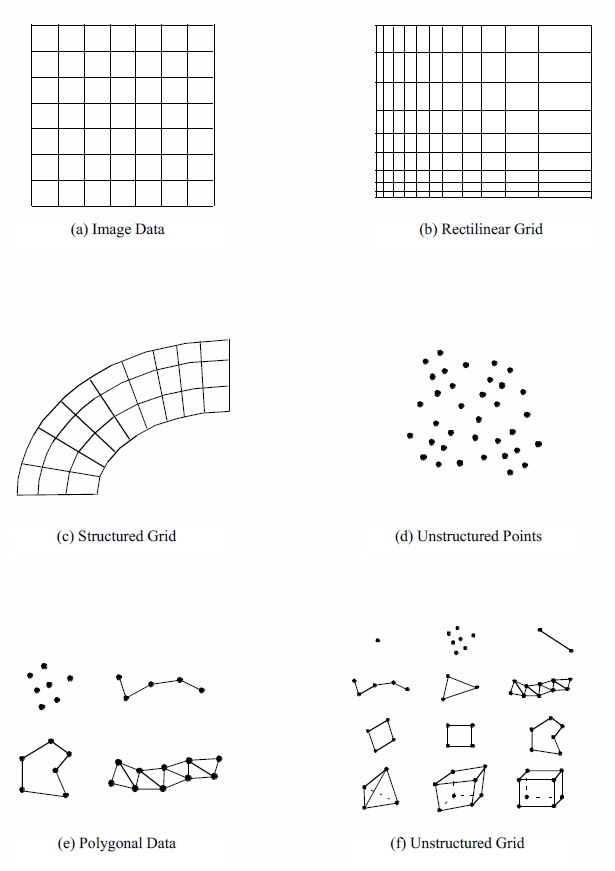
\includegraphics[width=0.8\textwidth]{Figure5-7}
	\caption{Dataset types. The unstructured grid consists of all cell types.}
	\label{fig:Figure5-7}
\end{figure}

\begin{figure}[!htb]
	\centering
	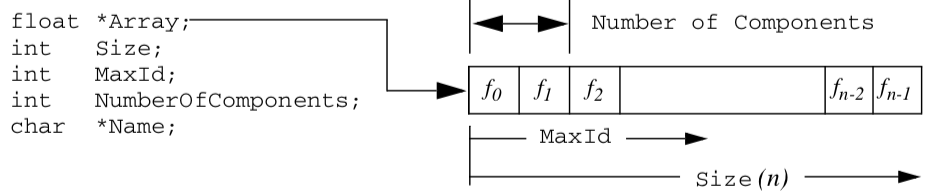
\includegraphics[width=0.8\textwidth]{Figure5-8}
	\caption{Implementation of contiguous array. This example is a fragment of the class definition vtkFloatArray.}
	\label{fig:Figure5-8}
\end{figure}

\begin{figure}[!htb]
	\centering
	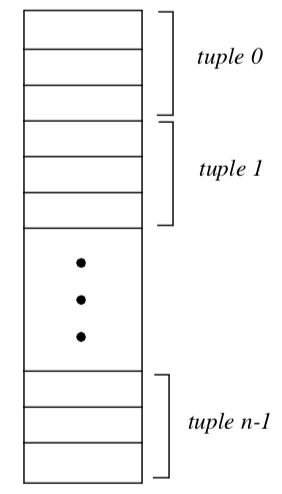
\includegraphics[width=0.8\textwidth]{Figure5-9}
	\caption{Data array structure. In this example, each tuple has 3 components.}
	\label{fig:Figure5-9}
\end{figure}

\begin{figure}[!htb]
	\centering
	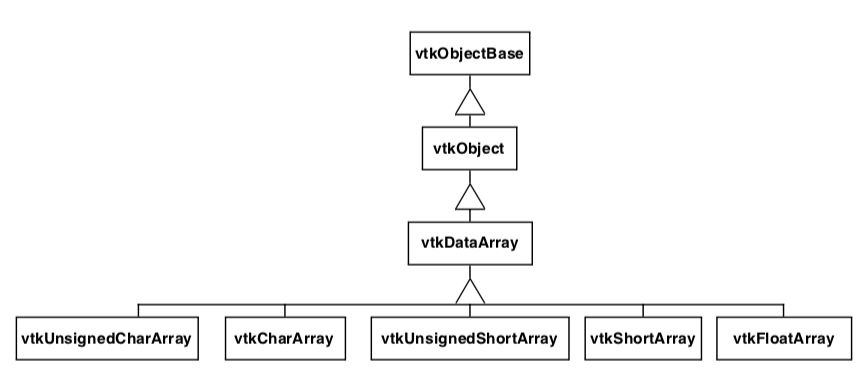
\includegraphics[width=0.8\textwidth]{Figure5-10}
	\caption{Data array object diagram. vtkDataArray is an abstract base class. Subclasses of vtkDataArray implement type specific representation and operations. Note: not all concrete data array subclasses are shown in this diagram.}
	\label{fig:Figure5-10}
\end{figure}

\begin{figure}[!htb]
	\centering
	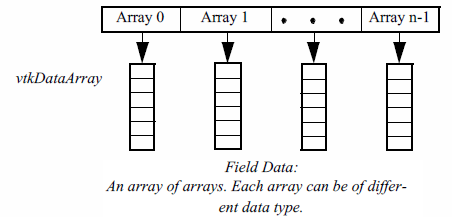
\includegraphics[width=0.8\textwidth]{Figure5-11}
	\caption{Data object representation as field data. A field can be represented as an array of arrays. Each array has a specified type, length, tuple size, and name. The association of a data array with points or cells, and its labeling as a particular attribute type, forms point and cell attribute data.}
	\label{fig:Figure5-11}
\end{figure}

\begin{figure}[!htb]
	\centering
	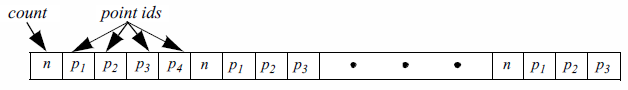
\includegraphics[width=0.8\textwidth]{Figure5-12}
	\caption{vtkCellArray structure to represent cell topology.}
	\label{fig:Figure5-12}
\end{figure}

\begin{figure}[!htb]
	\centering
	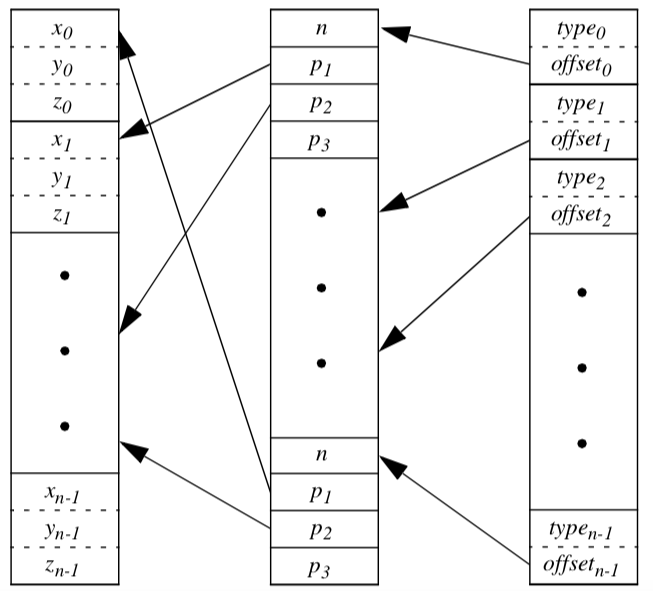
\includegraphics[width=0.8\textwidth]{Figure5-13}
	\caption{The data structure of the class vtkUnstructuredGrid. (This is a subset of the complete structure. See Chapter 8 for complete details.}
	\label{fig:Figure5-13}
\end{figure}

\begin{figure}[!htb]
	\centering
	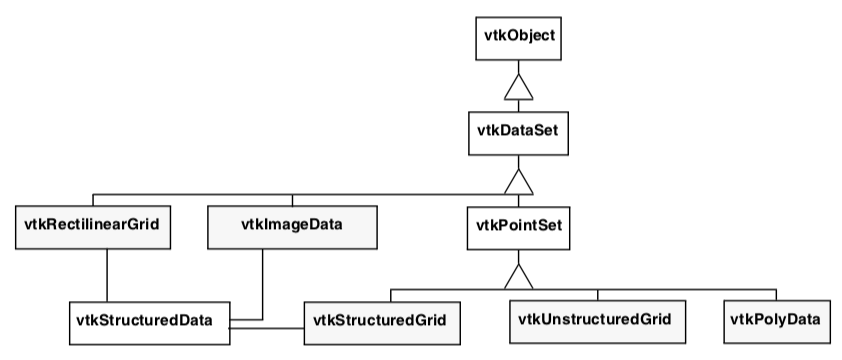
\includegraphics[width=0.8\textwidth]{Figure5-14}
	\caption{Dataset object diagram. The five datasets (shaded) are implemented in VTK.}
	\label{fig:Figure5-14}
\end{figure}

\begin{figure}[!htb]
	\centering
	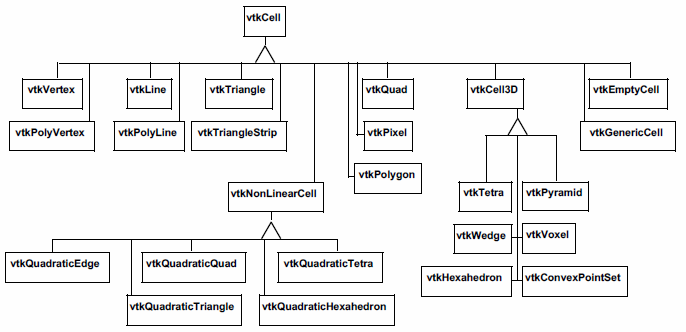
\includegraphics[width=0.8\textwidth]{Figure5-15}
	\caption{Object diagram for twenty concrete cell types in VTK. vtkEmptyCell represents NULL cells. vtkGenericCell can represent any type of cell. Three-dimensional cells are subclasses of vtkCell3D. Higher order cells are subclasses of vtkNonLinearCell.}
	\label{fig:Figure5-15}
\end{figure}

\begin{figure}[!htb]
	\centering
	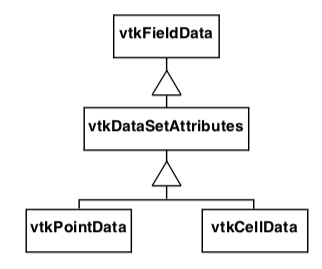
\includegraphics[width=0.8\textwidth]{Figure5-16}
	\caption{Inheritance hierachy for representing data set attributes.}
	\label{fig:Figure5-16}
\end{figure}

\begin{figure}[!htb]
	\centering
	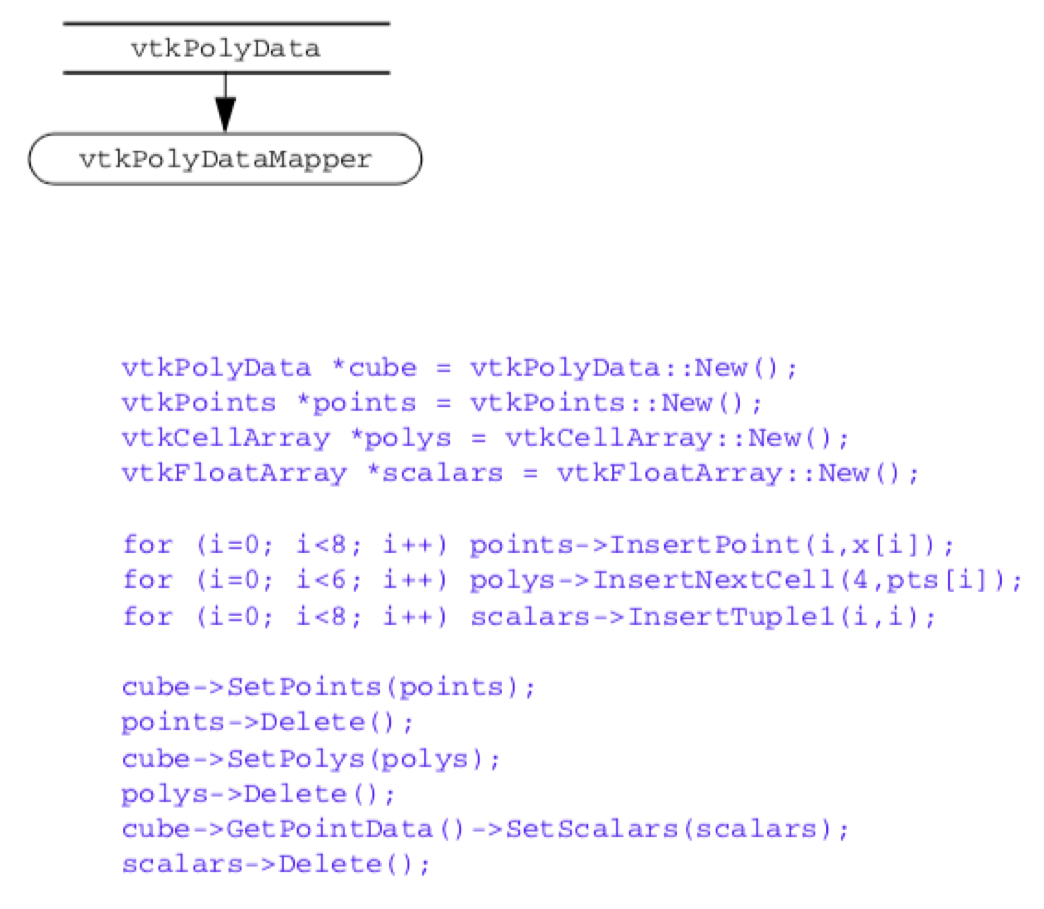
\includegraphics[width=0.8\textwidth]{Figure5-17}
	\caption{Creation of polygonal cube.}
	\label{fig:Figure5-17}
\end{figure}

\begin{figure}[!htb]
	\centering
	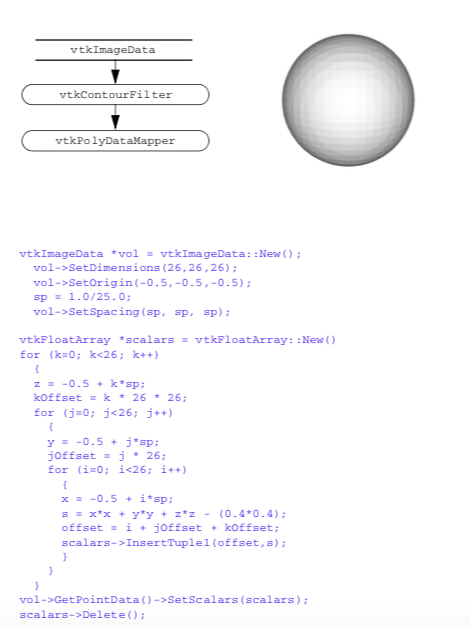
\includegraphics[width=0.8\textwidth]{Figure5-18}
	\caption{Creating a image data dataset. Scalar data is generated from the equation for a sphere. Volume dimensions are $26^3$.}
	\label{fig:Figure5-18}
\end{figure}

\begin{figure}[!htb]
	\centering
	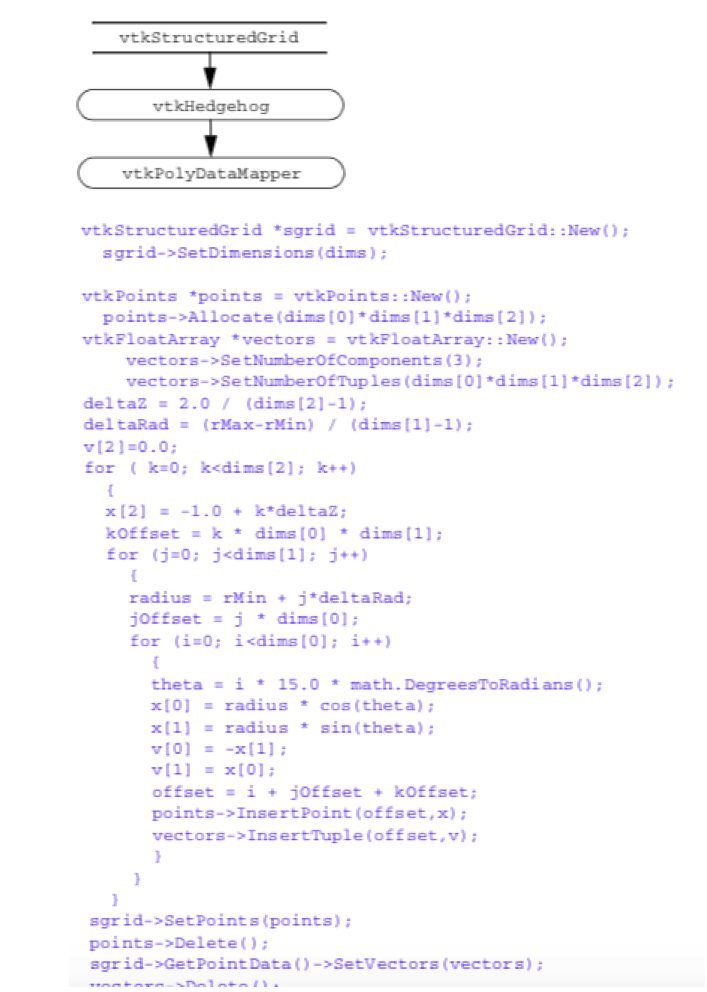
\includegraphics[width=0.8\textwidth]{Figure5-19}
	\caption{Creating a structured grid dataset of a semi--cylinder. Vectors are created whose magnitude is proportional to radius and oriented in tangential direction.}
	\label{fig:Figure5-19}
\end{figure}

\begin{figure}[!htb]
	\centering
	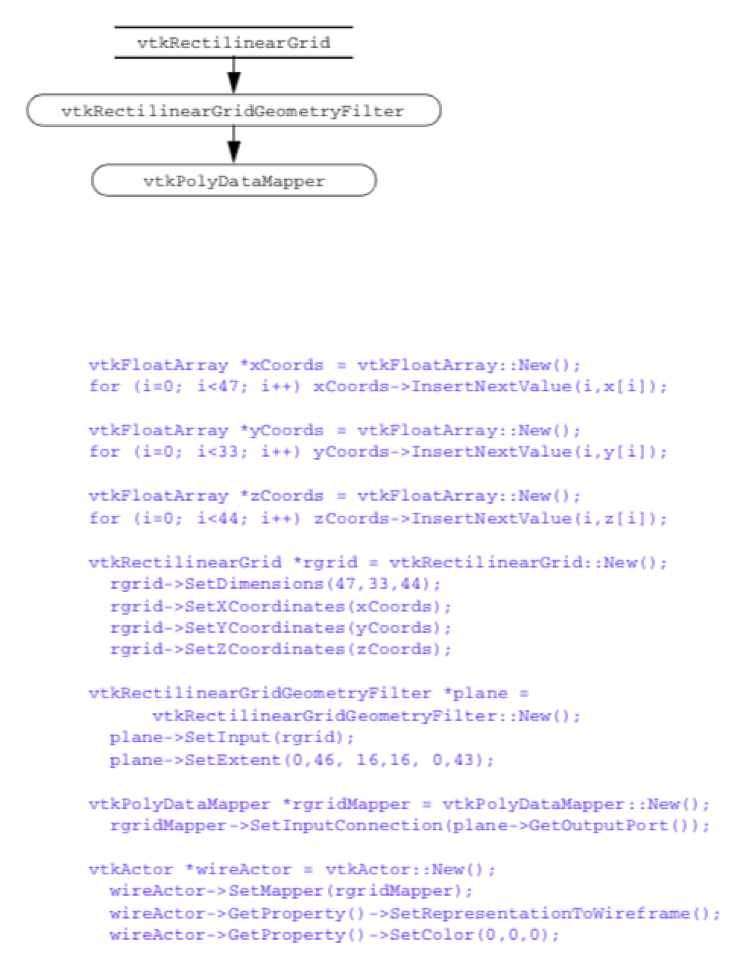
\includegraphics[width=0.8\textwidth]{Figure5-20}
	\caption{Creating a rectilinear grid dataset. The coordinates along each axis are defined using an instance of vtkDataArray.}
	\label{fig:Figure5-20}
\end{figure}

\begin{figure}[!htb]
	\centering
	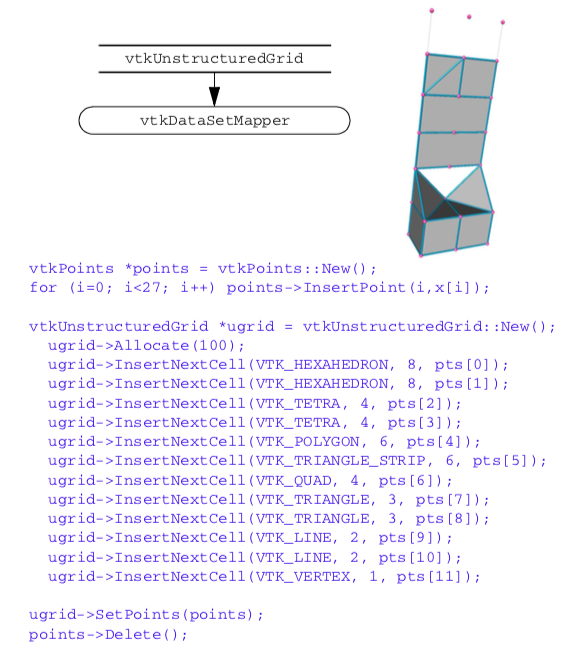
\includegraphics[width=0.8\textwidth]{Figure5-21}
	\caption{Creating a structured grid dataset of a semicylinder. Vectors are created whose magnitude is proportional to radius and oriented in tangential direction.}
	\label{fig:Figure5-21}
\end{figure}



\section{Bibliographic Notes}

A variety of representation schemes have been proposed for each dataset type described here. These schemes vary depending on design goals. For example, even the simple volume representation has been implemented with other more complex schemes such as run-length encoding and octrees \cite{Bloomenthal88}. A description of more general representation schemes is available in \cite{Haber91}, the AVS field model \cite{AVS89}, and the compact cell structure \cite{Schroeder94}. An overview of dataset types can be found in \cite{Gelberg90}. Some structures for those mathematically oriented can be found in \cite{Brisson90} and \cite{Poluzzi93}. Haimes \cite{VISUAL3} describes an efficient data structure for unstructured grid visualization.

If you are interested in more details on finite element methods see the classic Zienkiewicz \cite{Zienkiewicz87} or \cite{Gallagher75}. Information about both finite difference and finite element methods is available in \cite{Lapidus82}.

\printbibliography


\section{Exercises}

\begin{enumerate}

\item Consider a pixmap of dimensions 1002. Compare the memory requirements to represent this data using:

\begin{enumerate}

	\item an image dataset,

	\item a structured grid dataset,

	\item a polygonal mesh of quadrilaterals,

	\item an unstructured grid of quadrilateral cells,

	\item and a triangle strip mesh of 100 strips of 200 triangles each.

\end{enumerate}

\item Consider a volume of dimensions 1003. Compare the memory requirements to represent this data using:

\begin{enumerate}

	\item an image dataset,

	\item a structured grid dataset,

	\item and an unstructured grid of hexahedral cells.

\end{enumerate}

\item Develop a representational scheme for a rectilinear grid. How does this compare (in memory requirement) to a structured grid?

\item Consider a volume of dimensions 1003. Compute the memory requirements for the following point attribute types:

\begin{enumerate}

	\item unsigned character scalars (1 byte per scalar),

	\item float scalars (4 bytes per scalar),

	\item float vectors,

	\item and double-precision tensors (3x3 tensors).

\end{enumerate}

\item List three examples of scalar data.

\item List three examples of vector data.

\item List three examples of tensor data.

\item Is it possible to have more than one scalar field in a dataset? If so, how would this information be represented?

\item  A common method to represent cell connectivity is to list point ids with the last id negated. For example, triangle (8,7,3) would be represented (8,7,-3). The negative index represents end of cell definition. What are the advantages and disadvantages of this scheme as compared to the VTK cell array structure?

\item  How many different ways can a hexahedral cell be decomposed into tetrahedron? Are there compatibility issues between neighboring hexahedra?

\item Write a program to create and display a structured grid in the form of a hollow cylinder (i.e., cylinder with a hole through it).

\item Write a program to create and display an unstructured grid in the form of a hollow cylinder.

\item Write a program to create and display a polygonal octahedron.

\end{enumerate}
